\documentclass[conference]{IEEEtran}
\usepackage{cite}
\usepackage{amsmath,amssymb,amsfonts}
\usepackage{algorithmic}
\usepackage{graphicx}
\usepackage{textcomp}
\usepackage{xcolor}
\usepackage{url}

\def\BibTeX{{\rm B\kern-.05em{\sc i\kern-.025em b}\kern-.08em
    T\kern-.1667em\lower.7ex\hbox{E}\kern-.125emX}}
\begin{document}

\title{
    Indor Robot Pose Estimation
}

\author{
    Eduardo Henrique Basilio de Carvalho
}

\maketitle

\begin{abstract}
    This report presents the development and evaluation of various algorithms for estimating the pose of the Indor robot using laser and odometry data. Different filtering techniques, including the Unscented Kalman Filter, Extended Kalman Filter, and Particle Filter, were implemented and compared. The performance of each method was assessed based on accuracy and computational efficiency. Hyperparameter optimization was conducted to enhance the models' performance. The results highlight the importance of the model selection for effective pose filtering in the studied problem.
\end{abstract}

\section{Introduction} \label{sec:introduction}

In the provided problem, the odometry data exhibits a noticeable drift, as discussed in Section \ref{sec:odometry}. This drift leads to a significant discrepancy between the odometry estimates and the reference data, which can adversely affect the overall pose estimation accuracy. While laser data has the potential to mitigate this drift by providing more accurate position information, it is important to note that laser readings are often subject to noise and other environmental factors. Consequently, relying solely on laser data for robot localization presents its own challenges. The integration of both odometry and laser data is essential for achieving a robust and reliable pose estimation, as it allows for the correction of odometry drift while leveraging the strengths of each data source.

Since the trajectory spans across several meters and the laser model exhibits dependency on the map structure, linear filtering approaches prove insufficient for achieving adequate pose estimates. The spatial variation of the environment introduces nonlinearities in the measurement model that cannot be adequately captured by linear filters such as the standard Kalman Filter. Consequently, nonlinear filtering techniques are necessary to properly account for these dynamics and provide reliable pose estimation. These advanced filtering methods are discussed in detail in Section \ref{sec:filters}.

\section{Map} \label{sec:map}

Figure \ref{fig:map} illustrates the environment in which the robotic experiments were conducted. The map is represented as a binary occupancy grid, where white pixels denote free space accessible to the robot, while black pixels represent obstacles and walls that must be avoided during navigation. This map representation is essential for the laser model, as it defines the expected measurement relationships between the robot's pose and the corresponding laser range observations.

\begin{figure}[htbp]
    \centerline{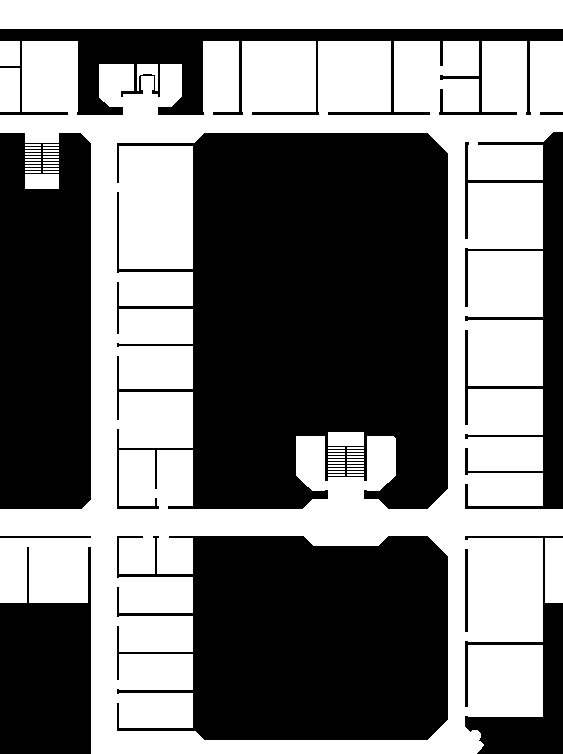
\includegraphics[width=\linewidth]{map.png}}
    \caption{Map of the environment where the Indor robot operates.}
    \label{fig:map}
\end{figure}

\subsection{Transformation to Data's Frame} \label{sec:transformation_to_data_frame}

The source material provides the map in conventional coordinates with pixel-scale representation. However, since the experimental data is provided in a shifted, rotated, and scaled reference frame, several coordinate transformations were necessary to ensure consistency between the map and the data. The following transformations were applied in sequence:

\begin{enumerate}
    \item \textbf{Origin Centering:} The coordinate system was translated such that the origin $(0, 0)$ is positioned at the center of the map, rather than at a corner. This transformation is defined as:
    \begin{equation}
        x' = x - \frac{w}{2}, \quad y' = y - \frac{h}{2}
    \end{equation}
    where $w$ and $h$ are the width and height of the map in pixels, respectively.
    
    \item \textbf{Y-axis Inversion:} The $y$-axis was inverted to align with the data's coordinate convention, transforming the pixel coordinates from image space to a standard Cartesian frame:
    \begin{equation}
        y'' = -y'
    \end{equation}
    
    \item \textbf{Scale Conversion:} Pixel coordinates were converted to metric units using the provided scale factor $s$ (in meters per pixel):
    \begin{equation}
        x_m = s \cdot x', \quad y_m = s \cdot y''
    \end{equation}
    
    \item \textbf{Spatial Cropping:} The map was cropped to focus on the region of interest encompassing the experimental trajectory, reducing computational overhead while maintaining the necessary environmental context for laser-based localization.
\end{enumerate}

These transformations ensure that the map representation is consistent with the odometry and laser data frames, enabling accurate pose estimation throughout the experiment.

\section{Data} \label{sec:data}

The experimental data was initially provided in a single space-separated file, which contained various measurements and observations relevant to the pose estimation task. To enhance organization and facilitate subsequent processing, this data was systematically divided into three distinct comma-separated files. Each file corresponds to a specific type of data: reference data, laser measurements, and odometry readings.

This separation allows for more efficient data handling and processing, as each file can be independently accessed and manipulated according to its specific requirements. The reference data file contains the ground truth positions against which the estimated poses can be compared. The laser measurements file includes the range and bearing information captured by the robot's laser sensors, while the odometry readings file records the robot's estimated position based on its movement and wheel encoders.

If we denote the original data as \( D \) and the separated files as \( D_{ref} \), \( D_{laser} \), and \( D_{odom} \), we can express the separation process as follows:

\[
D = \{D_{ref}, D_{laser}, D_{odom}\}
\]

This structured approach not only improves clarity but also streamlines the data preprocessing steps that follow, ensuring that each dataset can be effectively utilized in the filtering and estimation algorithms discussed in subsequent sections.

\subsection{Reference} \label{sec:reference}

The reference data is provided in the global frame with absolute values, which is crucial for accurate pose estimation. This dataset consists of three columns: the first column contains the \( x \) coordinates, representing the robot's position along the horizontal axis; the second column contains the \( y \) positions, indicating the robot's position along the vertical axis; and the third column contains the yaw angles, denoted as \( \theta \), which represent the orientation of the robot in radians.

Mathematically, we can express the reference data as a set of tuples \( R \) defined as follows:

\[
R = \{(x_i, y_i, \theta_i) \mid i = 1, 2, \ldots, N\}
\]

where \( N \) is the total number of observations. Each tuple \( (x_i, y_i, \theta_i) \) corresponds to a specific time step \( i \) and provides essential information for evaluating the performance of the pose estimation algorithms. The yaw angle \( \theta_i \) is particularly important as it allows for the transformation of the robot's pose from the global frame to the local frame, facilitating the integration of laser and odometry data in subsequent filtering processes.

\begin{figure}[htbp]
    \centerline{
\includegraphics[width=\linewidth]{reference_trajectory.png}}
    \caption{Reference trajectory of the Indor robot in the global frame.}
    \label{fig:reference_trajectory}
\end{figure}

Figure \ref{fig:reference_trajectory} presents a visual representation of the reference data plotted over the map of the environment. This overlay allows for a direct comparison between the estimated poses derived from the filtering algorithms and the ground truth positions provided in the reference dataset. 

Mathematically, we can denote the reference positions as \( R = \{(x_i, y_i, \theta_i) \mid i = 1, 2, \ldots, N\} \), where each tuple corresponds to the robot's position and orientation at discrete time steps. The plotted reference trajectory serves as a benchmark for evaluating the accuracy of the pose estimation methods employed in this study.

The visualization not only highlights the trajectory of the Indor robot but also emphasizes the spatial relationship between the robot's estimated poses and the obstacles present in the environment. This context is crucial for understanding the performance of the filtering techniques, as it illustrates how well the algorithms navigate through the mapped space while adhering to the constraints imposed by the environment.

In the subsequent sections, we will analyze the discrepancies between the reference data and the estimated poses, providing insights into the effectiveness of the various filtering approaches utilized in this research.

\subsection{Laser} \label{sec:laser}

The laser data comprises 360 columns, each corresponding to a single laser sensor reading. These sensors are angularly displaced by 0.5 degrees from one another, collectively covering the 180-degree frontal hemisphere of the robot. Mathematically, the angular coverage can be expressed as:

\begin{equation}
    \Delta\phi = 0.5\deg, \quad \Phi_{total} = 360 \times 0.5\deg = 180\deg
\end{equation}

where $\Delta\phi$ denotes the angular separation between adjacent sensors and $\Phi_{total}$ represents the total angular coverage.

Each sensor returns a range measurement in meters, representing the distance to the nearest obstacle detected in its corresponding direction. These measurements are expected to fall within the range $[0, 8]$ meters, defining the operational range of the laser scanner. The laser data can be represented as a vector of measurements $L$ at each time step:

\[
L = \{r_j \mid r_j \in [0, 8] \text{ m}, \quad j = 1, 2, \ldots, 360\}
\]

where $r_j$ denotes the range reading from the $j$-th sensor. This rich angular resolution provides detailed geometric information about the robot's surroundings, which is essential for accurate position correction in the pose estimation algorithms discussed in Section \ref{sec:laser_model}.

\begin{figure}[htbp]
    \centerline{
\includegraphics[width=\linewidth]{laser_scan.png}}
    \caption{Laser scan at a specific time step. Each red dot corresponds to a laser measurement.}
    \label{fig:laser_scan}
\end{figure}

Figure \ref{fig:laser_scan} illustrates a sample laser scan taken at a specific time step. In this figure, each red dot represents a laser measurement projected into the environment based on the robot's current pose. The distribution of these measurements provides insight into the spatial configuration of obstacles around the robot, which is crucial for effective localization and navigation.

In the context of the robot's pose and laser range data, we can express the transformation of laser readings into global Cartesian coordinates mathematically. 

Let:

\begin{itemize}
    \item \( (x, y, \theta) \) represent the robot's position and orientation, where \( x \) and \( y \) are the coordinates in the global frame, and \( \theta \) is the heading angle.
    \item \( r_i \) denote the laser range measurement at angle \( \alpha_i \) relative to the robot's heading.
\end{itemize}

The global coordinates of the laser points can be computed as follows:

\begin{enumerate}
    \item For each laser reading, the global angle is given by:
    
    \begin{equation}
        \text{global\_angle}_i = \theta + \alpha_i
    \end{equation}

\item The Cartesian coordinates of the laser point in the global frame are then calculated using:

   \begin{align*}
   x_{\text{laser}, i} & = x + r_i \cdot \cos(\text{global\_angle}_i) \\
   y_{\text{laser}, i} & = y + r_i \cdot \sin(\text{global\_angle}_i)
   \end{align*}
\end{enumerate}

This transformation ensures that the laser readings, which are initially in polar coordinates relative to the robot's local frame, are accurately represented in the global Cartesian coordinate system. The filtering condition \( 0.1 < r_i < 8.0 \) ensures that only valid laser readings are considered for this transformation.

\subsection{Odometry} \label{sec:odometry}

The odometry data serves as a crucial component in understanding the robot's movement throughout the experiment. It provides the cumulative displacement of the robot from its initial pose, allowing for the assessment of its trajectory over time. Each row in the odometry dataset corresponds to the global displacement from the starting position to a specific moment in the experiment.

Mathematically, we can represent the odometry data as a set of tuples \( O \) defined as follows:

\[
O = \{(x_i, y_i, \theta_i) \mid i = 1, 2, \ldots, N\}
\]

where \( N \) is the total number of observations. In this representation, the first column contains the \( x \) coordinates, indicating the robot's position along the horizontal axis; the second column contains the \( y \) coordinates, representing the robot's position along the vertical axis; and the third column contains the yaw angles, denoted as \( \theta \), which indicate the orientation of the robot in radians.

The cumulative displacement can be expressed as:

\[
\Delta x = x_i - x_0, \quad \Delta y = y_i - y_0, \quad \Delta \theta = \theta_i - \theta_0
\]

where \( (x_0, y_0, \theta_0) \) represents the initial pose of the robot. This formulation allows for the calculation of the robot's position and orientation at any given time step \( i \) relative to its starting point.

It is important to note that the odometry data serves as the input to the odometry models discussed in Section \ref{sec:odometry_model}. Rather than providing a reference for evaluation, the odometry model functions as the \textit{process model} in the estimation techniques employed in this work. Specifically, the odometry model generates predictions of the robot's pose evolution that are subsequently corrected by the integration of laser measurements through the filtering algorithms. The predictions from the odometry model are refined by the filtering techniques to account for the accumulated drift and produce more accurate pose estimates. This correction mechanism is central to the effectiveness of the Unscented Kalman Filter, Extended Kalman Filter, and Particle Filter approaches discussed in Section \ref{sec:filters}.

\section{Data Preprocessing} \label{sec:data_preprocessing}

Before the main problem of pose estimation is addressed, the experimental data must undergo preprocessing to facilitate subsequent identification and filtering operations. The preprocessing steps are designed to extract a representative subset of the data that captures the essential dynamics of the robotic experiment while reducing computational burden. Formally, if we denote the complete dataset as $D = \{D_{ref}, D_{laser}, D_{odom}\}$ with $N$ total observations, the preprocessing aims to produce a reduced dataset $D' \subset D$ with $N' < N$ observations such that:

\begin{equation}
    \mathcal{C}(D') \ll \mathcal{C}(D)
\end{equation}

where $\mathcal{C}(\cdot)$ represents the computational cost of subsequent filtering and estimation operations, while maintaining sufficient fidelity to the original experimental characteristics.

The preprocessing strategy employed in this work comprises two main steps: data decimation, which reduces the sampling frequency to achieve computational efficiency, and trajectory trimming, which removes the initial and final segments of the trajectory that may contain noise or irrelevant movements. These operations are described in detail in the following subsections.

\subsection{Decimation} \label{sec:decimation}

Data decimation is performed to reduce the computational burden of subsequent filtering operations while preserving the essential dynamics of the robot's trajectory. The decimation process selects a subset of the original observations at regular intervals, effectively reducing the sampling frequency. If the original dataset contains $N$ observations sampled at frequency $f_s$, decimation with factor $d$ yields a reduced dataset with $N' = \lfloor N / d \rfloor$ observations sampled at frequency $f_s' = f_s / d$.

The decimation factor was determined through a systematic trial-and-error manual process. Various decimation ratios were tested by applying each factor to the complete dataset and subsequently visualizing the resulting reference trajectory overlaid on the environment map. This visual inspection approach allowed for qualitative assessment of how well the decimated trajectory preserved the essential characteristics of the original path. The selection criterion was to identify the highest decimation factor that yielded a trajectory sufficiently similar to the original, thereby minimizing data while maintaining fidelity to the experimental dynamics.

Following this evaluation procedure, a decimation factor of $d = 100$ was selected as the optimal compromise between computational efficiency and trajectory preservation. This factor reduces the dataset by two orders of magnitude, substantially decreasing the computational requirements for the filtering algorithms discussed in Section \ref{sec:filters}, while ensuring that the decimated trajectory adequately represents the robot's movement through the environment.

It is important to note that all figures and results presented throughout this document already reflect the application of this decimation factor. Consequently, the visualizations and quantitative analyses shown hereafter correspond to the reduced dataset with sampling frequency $f_s' = f_s / 100$.

\subsection{Trimming} \label{sec:trimming}

Trajectory trimming is performed to eliminate segments of the robot's path that may introduce noise or irrelevant movements, particularly at the beginning and end of the experiment. These segments often contain transient behaviors, such as manual positioning or stopping maneuvers, which do not contribute meaningfully to the analysis of the robot's steady-state navigation performance. By removing these portions of the trajectory, the focus is placed on the segments where the robot is actively navigating the environment, thereby enhancing the quality of the data used for filtering and estimation. The first 10 and last 50 observations were removed from the dataset, resulting in a trimmed trajectory that better represents the robot's operational behavior during the experiment.

\section{Laser Model} \label{sec:laser_model}



\section{Odometry Model} \label{sec:odometry_model}

\section{Filters} \label{sec:filters}

\subsection{Unscented Kalman Filter} \label{sec:unscented_kalman_filter}

\subsection{Extended Kalman Filter} \label{sec:extended_kalman_filter}

\subsection{Particle Filter} \label{sec:particle_filter}

\section{Hyperparameter Optimization} \label{sec:hyperparameter_optimization}

\section{Results} \label{sec:results}

\section{Conclusion} \label{sec:conclusion}

\appendix

\section{Linear Models on a Reduced Range} \label{sec:apdx_linear_models_on_a_reduced_range}

\subsection{Range} \label{sec:apdx_range}

\subsection{Laser Model} \label{sec:apdx_laser_model}

\subsection{Odometry Model} \label{sec:apdx_odometry_model}

\subsection{Results} \label{sec:apdx_results}

\begin{thebibliography}{00}

\bibitem{Aguirre2007}
L. A. Aguirre, \emph{Introdução à identificação de sistemas: técnicas lineares e não lineares aplicadas a sistemas — teoria e aplicação}, 3\textsuperscript{a} ed. Belo Horizonte: Editora UFMG, 2007. ISBN 8570412207.

\bibitem{scikit-learn}
F. Pedregosa, G. Varoquaux, A. Gramfort, V. Michel, B. Thirion, O. Grisel, M. Blondel, P. Prettenhofer, R. Weiss, V. Dubourg, J. Vanderplas, A. Passos, D. Cournapeau, M. Brucher, M. Perrot and E. Duchesnay, “Scikit-learn: Machine Learning in Python,” \emph{Journal of Machine Learning Research}, vol. 12, pp. 2825-2830, 2011.

\bibitem{scikit-optimize}
T. Head, M. Kumar, H. Nahrstaedt, G. Louppe and I. Shcherbatyi, “scikit-optimize (skopt) v0.8.1,” Python package, 2020. [Online]. Available: \url{https://github.com/holgern/scikit-optimize}.

\bibitem{FilterPy}
M. Carter, \emph{FilterPy 1.4.4}. Python library for Kalman filtering and Bayesian estimation, 2022. [Online]. Available: \url{https://github.com/mjcarter95/FilterPy}.

\end{thebibliography}


\end{document}
